\chapter{Grundlagen}
\label{Grundlagen}

Dieses Kapitel stellt die für die weiteren Ausführungen notwendigen Begriffe und Systeme vor.
Entsprechend dem Inhalt dieser Arbeit werden generelle Grundlagen zu Informationssystemen und zur geografische Datenverarbeitung dargelegt.
Weiterhin werden verwendete Methoden und Systeme dargestellt.

Der zentrale Begriff des \Gls{gis} bedingt eine Auseinandersetzung mit Datenbanken und Informationssystemen.
Weiterhin ist die Mächtigkeit der zu untersuchenden Systeme abzugrenzen.
Dies erfolgt mit der Definition von Frameworks und von \Gls{gis}.
%Zentral für die Arbeit ist die Klärung des Begriffes Framework.
Ein Framework ist eine Softwareumgebung zur wiederverwendbaren Herstellung einer Struktur oder Anwendung.
Entweder werden Anwendungen mit Frameworks vervollständigt oder aus daraus erstellt.
In dieser Arbeit dienen Frameworks, oder auch Ordnungsrahmen genannt, zur Lösung spezieller Aufgaben und sind somit domänenspezifische Frameworks.
Das heißt, dass notwendige Funktionen und Strukturen zur Lösung von speziellen Aufgaben bereits vorhanden sind, die konkreten Lösungen müssen jedoch mit Hilfe des Frameworks erstellt werden.
Die am Ende dieses Kapitels vorgestellten Frameworks zählen zu Alternativen des relationalen Datenbankmodell, weshalb dieser und dazugehörige Begriffe definiert werden.

\section{Datenbankmanagementsysteme}

Grundlegende Kenntnisse zu Datenbankmanagementsystemen und deren Mechanismen sind Voraussetzung für das Verständnis von Informationssystemen.
Dazu zählt Sharding.
Bei Sharding wird eine Relation in disjunkte Partitionen aufgeteilt, die auf verschiedenen Datenträgern gespeichert werden.
Vorteile dieser Methode sind Anfrageoptimierung durch Auslastung der Partitionen, Vereinfachung der Administration der Partitionen und parallele Verarbeitung (vgl. \cite[S.296]{book:kudrass}).
Dies setzt einen auf dieser Weise angepassten Query-Planer des \Gls{dbms} voraus.
Nach Kudraß wird nach drei Arten unterschieden.
Konkret sind das Bereichspartitionierung, Round-Robin-Partitionierung und Hash-Partitionierung.

Eine Erweiterung des aus \Gls{acid} bekannten Transaktionsmanagement ist \Gls{mvcc}, welches im Framework Postgres-XL zum Einsatz kommt.
In grundlegenden relationalen Systemen werden Transaktionen verzögert oder sogar gesperrt, um Konsistenz und Isolation zu gewährleisten.
\Gls{mvcc} erhöht die Effizienz des  blockierenden Verhaltens.
Dabei werden von jedem Objekt mehrere Versionen verwaltet.
Neue Versionen entstehen durch Änderungen einer anderen.
Eine Transaktion verwendet die zu Transaktionsbeginn aktuelle Version.
Dadurch werden die allgemeinen Sperrverfahren (siehe \cite[S.266 ff.]{book:kudrass}) verbessert, indem lesende Transaktionen sich nicht gegenseitig blockieren und schreibende- gegen lesende Transaktionen nicht mehr synchronisiert werden müssen. (vgl. \cite[S.270]{book:kudrass})

Da in dieser Arbeit verteilt arbeitende Frameworks untersucht werden, ist die Definition dieses Begriffes notwendig.
Nach \cite[S.394]{book:kudrass} wird bei einem Mehrrechner-Datenbanksystem (MDBS) die Datenbankverwaltungsfunktionen auf mehreren Prozessoren bzw. Rechnern ausgeführt.
Kudraß ergänzt dies durch folgende Unterscheidungen:\\
Ein \Gls{dbms} befindet sich auf eng gekoppelter Multiprozessor-Umgebung, was als shared everything bezeichnet wird.
Erfolgt die Verarbeitung durch mehrere Rechner mit jeweils einem \Gls{dbms}, wobei der Externspeicher unter den beteiligten Rechnern partitioniert ist, wird es shared nothing genannt.
Bei shared disk handelt es sich um mehrere lokal angeordnete, lose oder nah gekoppelte Rechner mit je einem \Gls{dbms} und einer gemeinsamen Speicherzuordnung.
Lokal verteilte Systeme werden als parallele Datenbanksysteme bezeichnet.
Ein Spezialfall stellen verteilte Datenbanksysteme dar.
\cite[S.398]{book:kudrass} beschreibt Verteilte Datenbanksysteme (VDBS) als geografisch verteilte shared nothing Systeme mit homogenen lokalen DBMS, die gemeinsam ein globales konzeptionelles Datenbankschema unterstützen.
Dagegen sind förderierte Datenbanksysteme (FDBS) ebenfalls geografisch verteilte shared nothing systeme, wobei die beteiligten lokalen DBMS eine höhere Autonomie aufweisen, d.\,h. dass jeweils eine eigene lokale Datenbank mit lokalem Datenbankschema vorliegt.


\section{Verarbeitung raumbezogener Daten}
%spatial mit verwenden - definieren: raumbezogen
Diese spezielle Form der Datenverarbeitung berücksichtigt geografische und topologische Eigenschaften.
Diese sind nach der Art und deren Bezug zueinander zu unterscheiden.
Der in diesem Zusammenhang in der englischen Literatur verwendete Begriff \glqq{}spatial data\grqq\ wird als \glqq{}räumliche Daten\grqq\ ins deutsche übersetzt, weshalb das Attribut räumlich nachfolgend raumbezogen ersetzt.

\subsection{Räumliche Bezugssysteme}
Entsprechend \cite[S.506]{book:kudrass} erlauben räumliche Bezugssysteme die Interpretation der gespeicherten Koordinaten als Beschreibung von Lage- und Ausdehnungsinformationen in einem Datenraum. Ein räumliches Bezugssystem besteht aus einem Koordinatensystem, einem Geltungsbereich und Angaben, die es erlauben, Daten aus unterschiedlichen Koordinatensystemen auf ein globales System abzubilden.
Lange ergänzt die allgemeine Definition von Kudraß indem er eine Unterscheidung der Koordinatensysteme nach kartesisch, homogen, Kugeltransformation und Ellipsoidentransformation durchführt, wobei den kartesischen einer hoher Stellenwert zugegordnet wird (vgl. \cite[S.141 ff.]{book:gi-theopluspraxis3}).

Allen Bezugssystemen wird zur Identifikation ein weltweit eindeutiger Code zugeordnet.
Dieser ist ein von der \Gls{epsg} vergebener so genannter \Gls{epsg-code}.
Das auf einem Ellipsoiden basierende Bezugssystem World Geodetic System von 1984 (WGS84) mit dem EPSG Code EPSG:4326\footnote{EPSG:4326: \url{http://spatialreference.org/ref/epsg/wgs-84/}} wird von der Agri~Con verwendet.


\subsection{Räumliche Objekte}
Lange definiert räumliche Objekte bzw. Geoobjekte als Elemente die zusätzlich zu ihrer Sachinformationen geometrische und topologische Eigenschaften besitzen und zeitlichen Veränderungen unterliegen können. Dabei sind Geometrie, Topologie, Thematik und Dynamik kennzeichnend.
Ein Geoobjekt enthält als Geometrie eine oder mehrere zwei- oder dreidimensionale Koordinaten, was die Lage, den Umfang und die Ausdehnung beschreibt.
Zur Topologie zählt de Lange Umgebungen, Nachbarschaften, Teilmengen und Überlagerungen.
Weiterhin werden Geoobjekte mit Sachinformationen gespeichert und je nach Anwendungsfall versioniert. (vgl. \cite[S.133]{book:gi-theopluspraxis3})


\subsubsection{Einfache Objekte}
Zu den einfachen Objekten zählen Punkte, Linien, Polygone, Multilines und Multipolygone.
Ein Punkt besteht aus einer zwei- oder dreidimensionalen Koordinate und beliebigen Sach-, Topologie- und Dynamikinformationen.
Mehrere Punkte bilden Linien.
Bildet eine Linie eine geschlossene Fläche, handelt es sich um einen Ring.
Ein Ring mit beliebigen Innenringen\footnote{Innenringe werden auch Inseln genannt.} ist ein Polygon.
Weiterhin können Gruppen von Linien und Polygonen gebildet werden und Multilines und Multipolygone bilden.

\subsubsection{Vektorenmodell}

Es besteht die Möglichkeit eine Menge von Punkten als Vektoren aufzufassen und daraus topologische Objekte entstehen zu lassen.
Um damit geografisch zu arbeiten ist eine Diskretisierung notwendig, d.\,h. die Vektoren sind miteinander in topologische Beziehung zu setzen.

\subsubsection{Rastermodell}
Ein Raster löst einen rechteckigen Bereich mit in einem Koordinatensystem gleichmäßig angeordneten quadratischen Bildelementen bzw. Pixeln fester Größe auf.
Geodaten werden ergo mit einer indizierten Matrix abgebildet.
Ein geografischer Punkt wird näherungsweise durch ein einzelnes Pixel dargestellt.
Linienzüge werden durch entsprechende Anordnungen zusammenhängender Pixel angenähert erfasst.
Diese können dann z.\,B. durch Folgen von Indexpaaren (Zeile, Spalte) der zugehörigen Pixel beschrieben werden.
Eine Fläche ist ebenfalls durch zusammenhängende Pixel darstellbar.
Somit sind keine weiteren Zusatzinformationen zur Modellierung von Flächen wie im Vektormodell notwendig. (vgl. \cite[S.136]{book:gi-theopluspraxis3})
Ein dreidimensionales Raster heißt Voxel.

\subsection{Räumliche Operationen}
% Grundlagenbuch geoinformatik zu rate ziehen
Räumliche Operationen, welche in den zu betrachtenden Frameworks eingesetzt werden, sind Transformationen.
Dabei werden die Koordinatenreferenzsysteme, die Objekte und die topologischen Informationen geändert.
Graeme führt Beispiele solcher Transformationen tabellarisch auf, siehe Tabelle  \ref{table:spatialfunctions}.
\begin{table}[h]
\centering
\begin{tabular}{|c|c|c|C{4cm}|}
\hline
\textbf{Von/Nach} & \textbf{Punkte} & \textbf{Linien} & \textbf{Flächen} \\ \hline
\textbf{Punkte} & Interpolation & Contouring & Thiessen Polygone \\ \hline
\textbf{Linien} & Linienüberschneidung & Linienglättung & Pufferzonen \\ \hline
\textbf{Flächen} & \glqq{}sample at points\grqq & Mediale Achse & Wieder\-holungs\-proben\-nahme auf Flächen \\ \hline
\end{tabular}
\caption[Beispiele für räumliche Transformationen]{Beispiele für räumliche Transformationen nach \cite[S.139]{book:gisforgeoscientists}}
\label{table:spatialfunctions}
\end{table}
Darin werden ausgewählte Transformationen zwischen Objekten aufgeführt.
Es ist zu erwähnen, dass Transformationen nicht nur mit den aufgezeigten Objekten verwendet werden.
So ist die Interpolation auch für Punkte zu Linien möglich.
Für die folgenden Betrachtungen sind jedoch nur die Transformationen Interpolation und Contouring von Interesse.
In allen Transformationen werden Mittel der Statistik verwendet, da neben geografischen und topologischen Informationen auch Sachinformationen in die Berechnungen einbezogen werden, welche in die Transformation verändert übernommen werden.
Diese Verknüpfung von Statistik und räumlichen Operationen heißt Geostatistik.

%Geostatistik
In den weiteren Ausführungen wird kriging als Methode der Geostatistik verwendet.
Der Entwickler war Kriging, welcher diese Transformation zur Vorhersage von Goldvorkommen in Süd Afrika verwendete (vgl. \cite[S.317]{book:spatialdataanalysis}).
Entsprechend Akin und Simes nach \cite[S.76]{book:verarbeitungspatialdata} ist Kriging ein Schätzvorgang, der eine bestimmte Anzahl von Proben in einem Wichtungsprozess so einbezieht, dass die Schätzvarianz zu einem Minimum wird.
So wird ein Raster mit Schätzwerten erzeugt und daraus Konturlinien für die optische Darstellung erzeugt.
Kriging wird bei Agri~Con eingesetzt, um aus Punktdaten mit Sachinformationen Vektordaten mit geschätzten Sachinformationen zu erzeugen, wobei die Sachinformationen gewichtet werden und eine hohe Erwartungstreue der Schätzwerte gegeben ist.

\subsection{Geografisches Informationssystem}
\label{grundlagen:gis}
%Relevant hervorheben
Ein Informationssystem ist eine Softwareumgebung zur umfassenden Verwendung von Daten.
Es stellt Möglichkeiten der Erfassung, Speicherung und Verarbeitung zur Verfügung.
Außerdem können Daten analysiert, übertragen, angezeigt und gepflegt werden.
Alle Daten und Ergebnisse sind Gegenstand der Verwendung von Informationssystemen. (vgl. \cite[S.32]{book:kudrass})
Wird ein Informationssystem im geografischen Kontext benötigt, muss es für die speziellen Aufgaben angepasst oder gegen ein dafür vorgesehenes ausgetauscht werden.
Der spezielle Einsatz liegt darin begründet, dass die geometrischen und topologischen Informationen der Geodaten sich im Informationssystem widerspiegeln müssen.
Somit hat das System die topologischen Zusammenhänge zu berücksichtigen und die Daten bevorzugt optisch darzustellen.

Lange definiert \Gls{gis} ähnlich:
\begin{quote}
Im Mittelpunkt  der  Geoinformatik  stehen  mit den  Geoinformationssystemen raumbezogene Informationssysteme, die im Gegensatz zu den übrigen Informationssystemen Geoobjekte  der realen Welt modellieren und diese in ein digitales Informationssystem abbilden [...]. Die Gegenstände eines Geoinformationssystems  besitzen  wie  auch  bei  allen  anderen  Informationssystemen  eine 
Thematik (und Dynamik). Das Besondere bei Geoinformationssystemen ist, dass Geoobjekte darüber hinaus Geometrie und Topologie als implizite und untrennbare Bestandteile aufweisen!  Die Verarbeitung derartiger raumbezogener Informationen erfordert spezielle Werkzeuge bzw. Funktionen, die von den übrigen Informationssystemen nicht bereitgestellt werden [...]. \cite[S.337]{book:gi-theopluspraxis3}
\end{quote}
Die Klärung dieses Begriffes ist wichtig, da die zu untersuchenden Frameworks \Gls{gis} sind und anhand der Definition eines \Gls{gis} untersucht und bewertet werden.

%\subsection{GDAL}

\subsection{Java Bibliothek GeoTools}
\label{geotools}
GeoTools\footnote{GeoTools: \url{http://docs.geotools.org/}} ist eine in Java geschriebene Open Source Bibliothek, welche Standardkonforme Operationen zur Verarbeitung von geografischen Daten bereitstellt.
Diese ist Teil der Open Source Geospatial Foundation (OSGeo)\footnote{Open Source Geospatial Foundation: \url{http://www.osgeo.org/}}.
Sie wird von Java nahen Frameworks im Kontext von \Gls{gis} verwendet, sodass die Bewertung dieser Frameworks die Kenntnis über GeoTools voraus setzt.
Die Implementierung erfolgte nach Anforderungen des \Gls{ogc}, worauf beispielsweise Geometrien der \Gls{jts} unterstützt werden und die OGC Filter Encoding Spezifikation von Attributen und räumlichen Filtern verwendet wird (vgl. \cite{website:geotools}).
Eine detaillierte Auflistung der Funktionalitäten ist im Anhang \ref{appendix-B} zu finden.

\subsection{PostgreSQL mit Erweiterung PostGIS}
PostGIS\footnote{PostGIS: \url{http://postgis.org/}} ist eine geografische Erweiterung der Objekt-relationalen Datenbank \mbox{PostgreSQL}\footnote{PostgreSQL: \url{http://www.postgresql.org/}}.
PostgreSQL wird dabei um geografische Datentypen, geografische Indizes und Funktionen erweitert.
Konkret wird der Simple Feature Access Standard verwendet und um den Datentyp Raster und weitere Funktionen zur Datenverarbeitung erweitert. (siehe \cite{website:postgisdocu-opengis})
Somit kann mit SQL direkt mit geografischen Daten gearbeitet werden.
PostGIS ist ein Projekt der Refractions Research\footnote{Refractions Research: \url{http://www.refractions.net/}} Gruppe und steht unter der \Gls{gpl}v2.


\section{Alternativen zum relationalen Datenbankmodell}
\label{nosql}
Alternativen des relationalen Datenbankmodells werden unter dem Stichwort NoSQL zusammengefasst und dieses soll hier als Synonym dienen.
NoSQL ist ein Begriff, dessen Kontext die Abkehr von klassischen relationalen Systemen fordert oder zumindest ein Umdenken bestehender Strukturen, Vorgehen und Grundsätze anstrebt.
Dies wird durch andere Abfragesprachen, nicht relationale Datenbankmodelle oder Neudefinitionen von Begriffen wie der Konsistenz zum Ausdruck gebracht.
Zu den Gründen des Umdenkens zählen die im Web 2.0 anfallenden unstrukturierten Daten, welche kostengünstig persistiert und zugänglich gemacht werden müssen.
Dafür wurden herkömmliche relationale Systeme nicht konzipiert.
Die Menge an Daten und die geografische Verteilung dieser führte zur Einführung neuer Methoden und Prinzipien.
Der Ursprung wird in der Literatur verschieden hergeleitet, jedoch zählen immer Systeme mit einer anderen Abfragesprache als SQL und einfache Key Value Datenbanken zu den ersten Vertretern der NoSQL Bewegung.
Auf einer Messe zu aktuellen Trends im Datenbankbereich wurde der Begriff NoSQL zuerst öffentlich für Lösungen dieser Bewegung verwendet (vgl. \cite{website:originnosql}) und ist seitdem ein Sammelbegriff für eine hohe Anzahl an Systemen.
Einen Überblick der bestehenden Systeme stellt Edlich auf einer eigenen Homepage bereit.\footnote{Übersicht über NoSQL DBMS: \url{http://nosql-database.org/}}

In Bezug auf NoSQL kann \Gls{gis} wie in \ref{grundlagen:gis} definiert werden, jedoch muss das zugrunde liegende System nicht relational sein.
Im Rahmen dieser Arbeit ist mit \Gls{gis} ein System oder die Teilsysteme zur räumlichen Datenhaltung, Datenverarbeitung und Bereitstellung gemeint, unabhängig des zu Grunde liegenden Konsistenzbegriffes und der Abfragesprache.

\subsection{Kategorisierung}
Edlich unterscheidet NoSQL Datenbanken nach den vier unten aufgeführten Kategorien \cite{book:nosql-einfuehrung}.
Jedoch kann eine eindeutige Zuteilung nicht für jedes System erfolgen, da Prinzipien verschiedener Kategorien auf eines zutreffen können.

\subsubsection{Key Value Datenbank}
Key Value Datenbanken speichern Daten in Tupeln aus Schlüssel und Wert.
Der Key ist eine Zeichenkette oder ein Hashwert und der Datentyp von Value ist beliebig im Rahmen der Datentypen der Datenbank.
Der Datenzugriff erfolgt über den Key.
Es existiert keine einheitliche Abfragesprache.
Erste Datenbanken die zu NoSQL zugeordnet werden sind Key Value Datenbanken. Konkret DBM und BerkleyDB.
Aktuelle Vertreter sind Amazon Dynamo, Riak, Voldemort und Redis.
Diese Datenbanken eignen sich für heterogene Daten, horizontale Skalierung und Schemafreiheit, da diese einfach strukturierten Daten sich in keiner Relation auf Datenbankebene zueinander befinden.

\subsubsection{Dokumentenbasierende Datenbank}
Hierbei werden strukturierte Daten, hier Dokumente, unter einem Hash abgelegt und sind über diesen abrufbar.
Diese Dokumente sind im Großteil der dokumentenbasierten Datenbanken versioniert.
Häufige Formate sind \Gls{json}, \Gls{bson} und \Gls{yaml}.
Ziel ist dabei, schemafreie Daten zu speichern und den Zugriff zu skalieren.
Dabei sind zumeist keine Joins verwendbar.
Bekannte Vertreter sind MongoDB, CouchDB und Terrastore.

\subsubsection{Spaltenorientierte Datenbank}
Im Gegensatz zu zeilenorientierten Datenbanken legen spaltenorientierte Datenbanken ihre Werte, hier Attribute einer Tabelle, spaltenweise ab.
Dies eignet sich für \Gls{olap} und Data Warehouse, da Spalteneinfügungen kostengünstig sind und Garbage Collection effektiv ist.
Dagegen besteht ein hoher Aufwand beim Lesen und Schreiben von zusammengehörigen Spalten.

Googles Big Table erweitert diesen Ansatz und beschreibt es in dessen Paper wie folgt:
\begin{quote}
A  Bigtable  is  a  sparse,  distributed,  persistent  multi-dimensional sorted map. The map is indexed by a row key, column key, and a timestamp; each value in the map is an uninterpreted array of bytes. \cite[S.1]{paper:bigtable}
\end{quote}
Die mehrdimensionalen Tabellen oder Maps sind vom Format:\\
$n*[Domain / Keyspace]\ x\ [item / Column\ Family]\ x\ [Key\ x]*n*[key+Value]$\\
%Dans zeug dazu anschauen
Googles Ansatz wurde quelloffen in HBase und Cassandra umgesetzt. Die konkrete Implementierung von Google wurde jedoch nicht veröffentlicht.
HBase verwendet folgendes Format:
Pro Tabelle ein Zugriff auf Zeilen per Rowkey.
Diese Zeilen enthalten Column Familys oder Spalten, welche wiederum eine Map namens Column Qualifier mit Tupeln aus der Version als Schlüssel und ein Byte-Array als Wert besitzen (vgl. \cite[S.13]{ba:dan}).

\subsubsection{Graphenbasierte Datenbank}
Der bekannteste Vertreter der graphenbasierten Datenbanken ist Neo4J.
Alle Daten und deren Beziehungen werden in Form von Graphen persistiert.
Ein Graph besteht dabei aus Knoten und gerichteten Kanten.
Knoten sind dabei strukturierte Objekte und Kanten Beziehungen zwischen den Objekten.
Diese strukturierten Objekte sind Key Value Tupel.
Zur Abbildung verschiedener Beziehungen, können Kanten typisiert sein.
Somit lassen sich direkt Beziehungen zwischen Daten definieren, was sich für semantische Netze, Abbildungen von Beziehungen, Bioinformatik und Internetrouting eignet.
Diese Datenbanken sind nur optional mit einem Schema versehen und besitzen keine einheitliche Abfragesprache.
Auch sind laut Spezifikation keine Joins vorgesehen.


\subsection{Hadoop}
\label{hadoop}
% http://blog.samibadawi.com/2012/03/hive-pig-scalding-scoobi-scrunch-and.html
Hadoop\footnote{Apache Hadoop: \url{https://hadoop.apache.org/}} ist ein unter der Apache Lizenz 2.0 stehendes Java-Framework zur Datenhaltung und Verarbeitung von großen Datenmengen auf einem Verbund von mehreren Computern.
Es basiert auf MapReduce und dem Dateisystem HDFS.
Das \Gls{hdfs} ist ein verteiltes Dateisystem, welches keine besonderen Anforderungen an die Hardware stellt und für die Verwendung von mehreren hundert bis mehreren tausend Computern ausgelegt ist.
Die in einem verteilten System teilnehmenden Computer heißen Knoten.
Es besitzt eine hohe Fehlertoleranz und ist für den Einsatz auf kostengünstiger Hardware ausgelegt.
Hoher Datendurchsatz und die Verwendung großer Dateien\footnote{Eine Datei kann mehrere Gigabyte bis mehrere Terrabyte groß sein und wird in Blöcke gleicher Länge aufgeteilt.} sind wesentliche Merkmale. (vgl. \cite[S.3]{paper:hadoop})
Die Datei-Blöcke werden redundant auf die Knoten verteilt und sind mit Hilfe des Name-Node abrufbar (vgl. \cite[S.7]{ba:dan}).

Die verteilte Verarbeitung übernimmt MapReduce.
Der Name MapReduce stammt aus der funktionalen Programmierung, in welcher die Funktionen \glqq map\grqq \ und \glqq reduce\grqq \ zum Einsatz kommen.
So werden die Daten mit einer map-Funktion modifiziert gesammelt und mit reduce-Funktion aggregiert.
Ein Master weist die Daten und Funktionen den Slaves zu, in diesem Zusammenhang werden die Slaves Worker genannt.
Die Slaves führen die Funktionen mit den ihnen zugewiesenen Daten aus und speichern ihre Ergebnisse auf deren Festplatte ab.
Slaves sind dabei Threads oder exklusive physische Recheneinheiten.
MapReduce wurde von Google definiert.
In Abbildung \ref{fig:mapreduce} ist der beschriebene Ablauf dargestellt.
Bereits hierbei werden keine besonderen Anforderungen an die Hardware gestellt (vgl. \cite[S.3]{paper:mapreduce}).
%
\begin{figure}[h!]
\centering
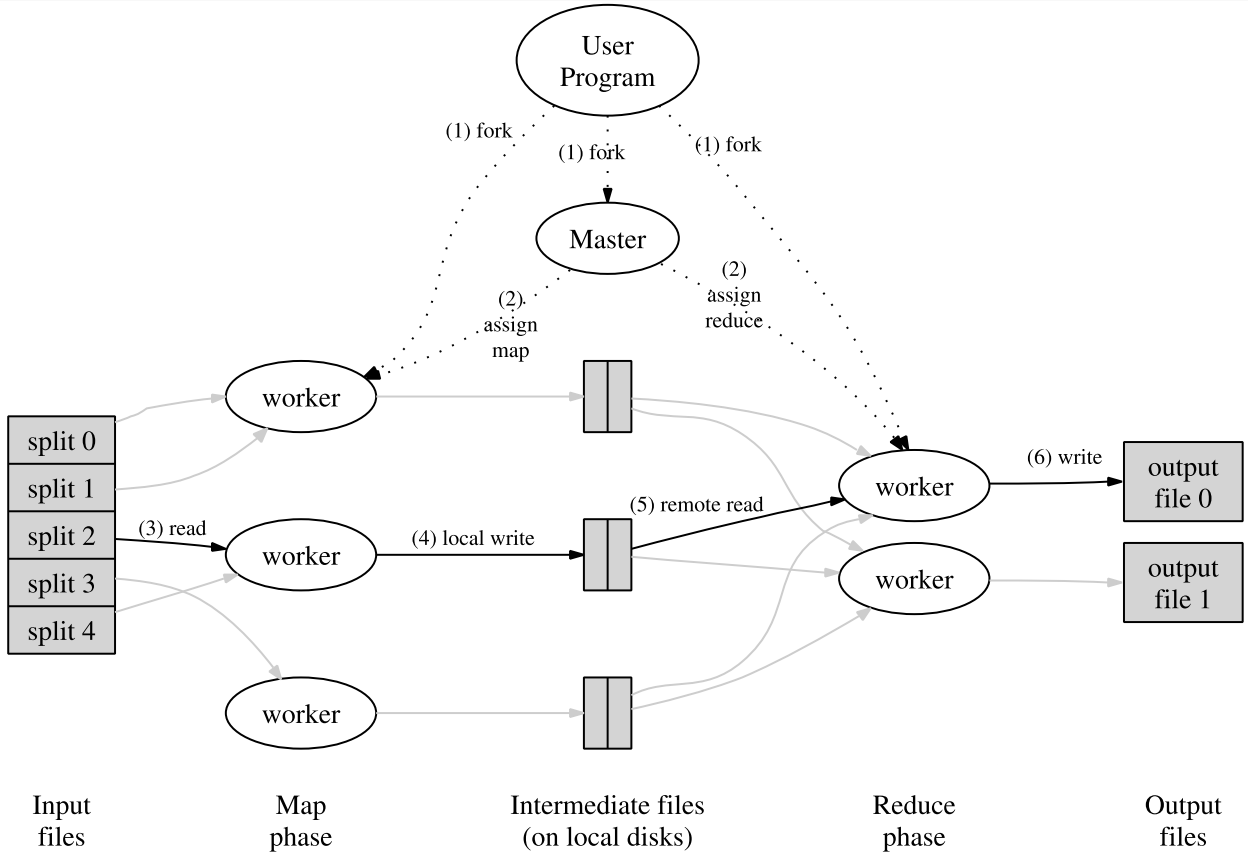
\includegraphics[width=\textwidth]{Abbildungen/mapreduce.png}
\caption[Übersicht der Ausführung von Googles MapReduce]{Übersicht der Ausführung von Googles MapReduce, Quelle: \cite{paper:mapreduce} S. 3}
\label{fig:mapreduce}
\end{figure}
Hadoop besitzt eine Master-Slave Architektur, wobei der Name-Node\footnote{Mit Name-Node ist der Master-Knoten gemeint, welcher in der Literatur auch das Synonym Jobtracker besitzt.} ankommende Anfragen bearbeitet und die Slave-Knoten organisiert.
Hadoop ist per API verwendbar und bietet sich somit zur Stapelverarbeitung an. %TODO belegen
Es wird meist nur als Grundgerüst verwendet und mit Datenbanken wie HBase, MongoDB oder PostgreSQL sowie mit Frameworks für die Nutzung wie Hive, \Gls{pig}, \Gls{spark} oder Scalding erweitert.

Gegenüber der Möglichkeit auf unterschiedlicher Hardware direkt und gleichzeitig mit Terrabyte großen Daten zu arbeiten, steht die Kritik das MapReduce eine hohe IO auf Festplatten der einzelnen Systeme erzeugt, da alle Zwischenergebnisse auf den Festplatten abgelegt und anschließend gelesen werden.

\subsection{Apache Accumulo}
\label{accumulo}
%https://en.wikipedia.org/wiki/Apache_Accumulo
Hierbei handelt es sich seit 2008 um ein Apache Projekt\footnote{Apache Accumulo: \url{https://accumulo.apache.org/}} und eine Java Open-Source Implementierung des BigTable Ansatzes von Google.
Es verwendet Hadoop, \Gls{zookeeper} und \Gls{thrift}.
Der BigTable Ansatz wird um Iteratoren, Zellenbezeichnungen, Constraints, physische Verteilungsmöglichkeiten einer dokumentbasierten Datenbank und die Unterstützung der gleichzeitigen Verwendung mehrerer HDFS Name-Nodes erweitert.
Weitere Funktionen sind folgende:
\newpage
\begin{itemize}
\item Verwendung mehrerer Master
\item Verwendung einer eigenen Zeitsynchronisation
\item Eingebaute temporäre Datenhaltung im Arbeitsspeicher
\item Bereitstellung von Testimplementierungen per API
\end {itemize}
Es stehen weiterhin verschiedene Erweiterungen zu Datenmanagement und Änderung des Ordnungsrahmens zur Verfügung. (vgl. \cite{website:accumulo_features})

\subsection{GIS GeoMesa}
GeoMesa\footnote{GeoMesa: \url{http://www.geomesa.org/}} ist eine unter Apache License Version 2.0 stehende geografische Datenbank der Firma LocationTech\footnote{LocationTech: \url{https://www.locationtech.org/}} mit den Möglichkeiten der verteilten Verarbeitung und Versionierung von geografischen Daten.
Dieses Framework ist in \Gls{scala} geschrieben.
Es erweitert Accumulo, unterstützt die GeoTools API und bietet ein Plugin für den Mapserver \Gls{geoserver} an.
Die Daten werden nach Geohash %\footnote{siehe \ref{geohash}}
verwaltet. (vgl. \cite{website:geomesaeclipse})

GeoMesa wird in Verbindung mit stream processing und batch processing verwendet.
Zur räumlichen Datenverarbeitung werden Scala Bibliotheken wie \Gls{jts} und GeoTools eingesetzt.
Vorrangig werden Vektordaten von GeoMesa verarbeitet, durch eine optionale Erweiterung sind auch Rasterdaten verwendbar.
Der Datenimport wird ingest genannt, erfolgt über die Kommandazeile und unterstützt die Datenformate CSV, TSV und SHP.
CSV, TSV, Shapefile, GeoJSON und GML können dagegen über den selben Weg exportiert werden.
Weiterhin erfolgt der Datenexport und -import über Scala. (vgl. \cite{website:geomesa-ingest})
GeoMesa ist konzipiert, um initial große Datenmengen per Ingest zu laden und diese anschließend mit Frameworks zur verteilten Datenverarbeitung wie \Gls{spark} und dafür vorgesehenen Bibliotheken zu verarbeiten.

\subsection{Postgres-XL}
\label{grundlagen:postgresxl}
Postgres-XL\footnote{Postgres-XL: \url{http://www.postgres-xl.org/overview/}} ist ein frei verfügbares Clustersystem für PostgreSQL unter der Mozilla Public License des Unternehmens TransLattice\footnote{TransLattice: \url{http://www.translattice.com/}}.
XL steht dabei für eXtensible Lattice, erweiterbarer Verbund.
Damit soll es ermöglicht werden, mit PostgreSQL verteilt Schreiboperationen zu skalieren sowie parallele Datenverarbeitung auf mehreren physischen und virtuellen Systemen gleichzeitig zu betreiben.
Es handelt sich um ein shared nothing Mehrrechner-Datenbanksystem.
Dafür wird zur verteilten Datenhaltung \Gls{acid} mit \Gls{mvcc}\footnote{\Gls{mvcc} ist bereits in PostgreSQL integriert} und zur parallelen Verarbeitung ein \Gls{mpp} Mechanismus eingesetzt.
Die Postgres-XL Umgebung nutzt mehrere PostgreSQL Instanzen und bietet Schnittstellen für alle Instanzen an. (siehe \cite{website:postgresxl-about})

Abbildung \ref{fig:postgresxl}\footnote{Link zur Abbildung: \url{http://www.postgres-xl.org/wp-content/uploads/2014/04/xl_cluster_architecture1.jpg}} verbildlicht den Aufbau.
Danach wird als erstes ein Load-Balancer angesprochen und es existieren mehrere GTM Instanzen. (siehe \cite{website:postgresxl-about})
Dies wird in der Dokumentation nicht belegt.
\begin{figure}[hp]
\centering
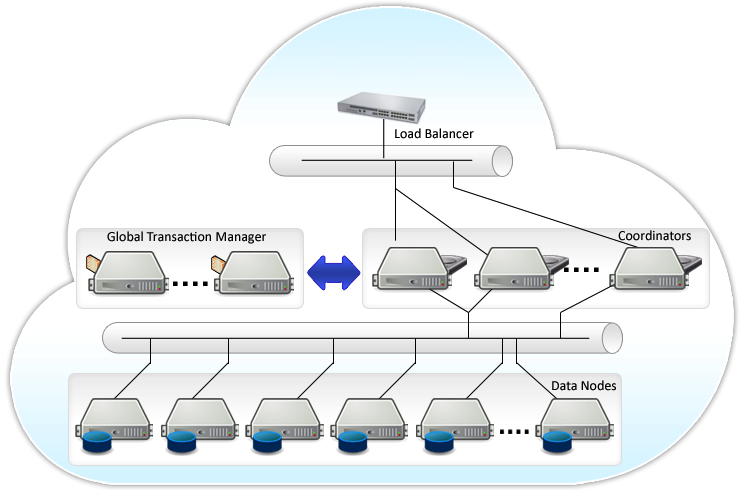
\includegraphics[width=.7\textwidth]{Abbildungen/postgresxl-structure.jpg}
\caption[Aufbau Postgres-XL]{Aufbau Postgres-XL, nach \cite{website:postgresxl-overview}}
\label{fig:postgresxl}
\end{figure}

Die Elemente sind nach \cite{website:postgresxl-about} wie folgt beschrieben:
\begin{description}
\item[Global Transaction Manager] Dient als Verwaltungselement der Transaktionen und realisiert \Gls{mvcc} über das System. Laut Dokumentation existiert genau ein GTM pro Cluster, um \Gls{mvcc}  mit einem globalen Kontext realisieren zu können. Der GTM wird von jeder Coordinator Instanz angesprochen. Es wird jedoch zusätzlich pro physischem Knoten des Clusters ein GTM-Proxy empfohlen, welcher die Anfragen an den GTM bündelt.
\item[Coordinator] Jeder Coordinator dient als Eintrittspunkt in den Cluster, ruft von der GTM Instanz pro SQL Statement eindeutige Transaktionsnummern und globale Informationen ab sowie formuliert Subquerys für die relevanten DataNodes entsprechend seines Query-Planers.
\item[Data Node] Diese Elemente sind PostgreSQL Instanzen, welche die konkreten Daten vorhalten und das Transaktionsmanagement an den GTM abgegeben haben. Die Datenbanken und Tabellen der DataNodes werden entweder per Partition verteilt oder repliziert. Anfragen können von verschiedenen Coordinators gleichzeitig in unterschiedlichen Sitzungen erfolgen. Auf Grund der Kapselung besitzt jeder Data Node seinen eigenen Kontext zur Transaktion.
\end{description}
Dabei besitzt jeder Coordinator und jeder DataNode einen ConnectionPool, welcher die Verbindungen verwaltet.
Veränderungen des Datenbankschemas werden auf alle Coordinators und DataNodes propagiert.
Es besteht jedoch die Möglichkeit einzelne DataNodes aus Relationen des Schemas zu entfernen.
Damit handelt es sich bei Postgres-XL um ein förderiertes Datenbanksystem.
Es wird analog einer PostgreSQL Installation angesprochen.
Zur Erhöhung der Ausfallsicherheit, besteht die Möglichkeit, für jedes Element im Cluster eine dazugehörige inaktive Instanz zu erzeugen, welche bei Ausfall der eigentlichen Instanz für diese einspringt.
Jedes Element im Cluster ist einzeln zu konfigurieren, was zu $ n*3+1 $ verschiedenen Konfigurationen bei $n$ DataNodes führt.
Zur Vereinfachung der Erstellung und Verwaltung eines Clusters sind neben den von PostgreSQL gelieferten Kommandozeilentools weitere durch Postgres-XL gegeben.
Zur Erstellung und Verwaltung eines Clusters kann pgxc-ctl eingesetzt werden.
Mit diesem Kommandozeilen Tool kann mit einer Konfigurationsdatei ein Cluster definiert sowie erstellt werden oder das Cluster mit einem Befehl um Knoten ergänzt werden.
%Das System wird somit analog einer PostgreSQL Instanz angesprochen.
Ebenso sind Erweiterungen wie PostGIS, DBLink oder PL/R installierbar.
Es ist zu erwähnen, dass die Version 9.2.34 keine Trigger unterstützt\footnote{Hinweis über fehlende Trigger in Postgres-XL: \url{http://files.postgres-xl.org/documentation/intro-whatis.html} Ergänzung 4} und der Transition Typ internal nicht verwendet werden kann.
%Verteilung findet nach Attribut statt, schließt aber bigint aus

\subsection{Array DBMS Rasdaman}
Rasdaman\footnote{Rasdaman: \cite{website:rasdaman.org}} ist ein Array-Datenbanksystem speziell zur Speicherung und Verarbeitung von Rasterdaten der rasdaman GmbH.
Es erweitert eine relationale Datenbank und wird mit  multi-dimensionalität der Daten, einer eigenen SQL ähnlichen Abfragesprache, Parallelisierung und Skalierbarkeit in beliebigen Maßstab sowie OGC konformen Diensten beworben.
Es ist als Client bzw. API unter der \Gls{lgpl} 3 und als Server unter der \Gls{gpl} 3 für Linux, MacOS und Solaris verfügbar.
Als OGC konforme Dienste werden WMS 1.3, WCS 2.0, WCS-T 1.4, WCPS 1.0 und WPS 1.0 bereitgestellt.
Die API kann in Java, C++ und über die eigene Abfragesprache rasql verwendet werden. (vgl. \cite{website:rasdamanogeo})
Der beschriebene Aufbau ist unter Abbildung \ref{fig:rasdaman}\footnote{Link zur Abbildung: \url{http://www.rasdaman.org/raw-attachment/wiki/Technology/wcps-stack.png}} dargestellt.
\begin{figure}[hp]
\centering
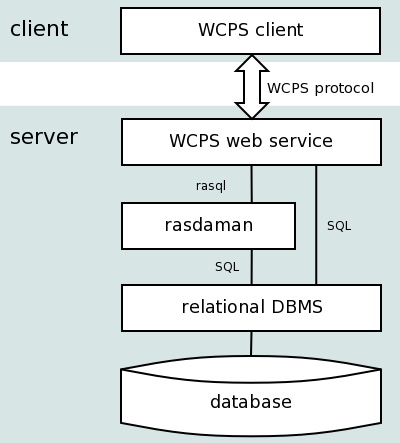
\includegraphics[width=.4\textwidth]{Abbildungen/rasdaman-aufbau.png}
\caption[Aufbau Rasdaman]{Aufbau Rasdaman}
\label{fig:rasdaman}
\end{figure}

Es besteht die Möglichkeit, Rasdaman zu einer bestehenden PostgreSQL Installation hinzuzufügen und direkten Datenaustausch zwischen den beiden Systemen zu ermöglichen.
Weiterhin kann Rasdaman in Verbindung mit der \Gls{gdal} verwendet werden.
Momentan existiert eine Community und eine Enterprise Variante. Dabei verfügt die Enterprise Variante über mehr Features wie beispielsweise Datenkomprimierung, Serververwaltung per Webbrowser, Laufzeitoptimierungen und verschiedene Datenbankschnittstellen.
Von der verwendeten Datenbank wird \Gls{blob} als Datenbankinterner Datentyp verwendet. (vgl. \cite{website:rasdamanowiki})